\documentclass[border=1mm]{standalone}
\usepackage[margin=2.5cm]{geometry}
\usepackage{graphicx,tikz,tikz-layers,amsmath}
\usetikzlibrary{decorations.markings,calc,positioning,arrows,shapes.geometric,arrows.meta}

% ========== 配色 ==========
\colorlet{feat}{blue!50!black}
\colorlet{head}{red!60!black}
\colorlet{linecol}{blue!40!black}

\begin{document}

\resizebox{\textwidth}{!}{
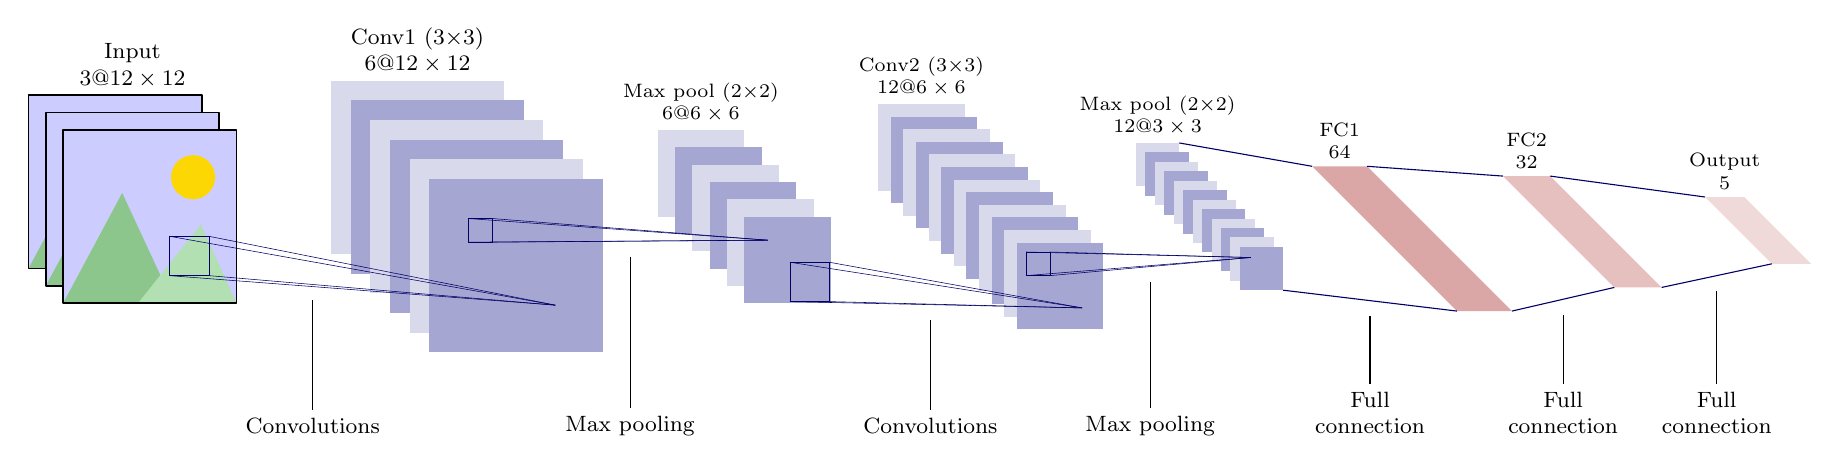
\begin{tikzpicture}[
    font=\footnotesize,
    scale=1,
    every node/.style={outer sep=0pt, inner sep=0pt, align=center},
    line join=round,
    >={Latex[length=2mm,width=1.5mm]}
  ]

  % ========== 可复用：单张风景画平面 ==========
  \newcommand{\picplane}[2]{%
    \begin{scope}[shift={(#1,#2)}]
      \fill[blue!20] (-1.1,-1.1) rectangle (1.1,1.1);                          % 天空
      \fill[yellow!75!orange] (.55,.5) circle (.28);                           % 太阳
      \fill[green!50!black!45] (-1.1,-1.1) -- (-.35,.3) -- (.3,-1.1) -- cycle; % 远山
      \fill[green!60!black!30] (-.15,-1.1) -- (.65,-.1) -- (1.1,-1.1) -- cycle;% 近山
      \draw[black, line width=.6pt] (-1.1,-1.1) rectangle (1.1,1.1);           % 边框
    \end{scope}
  }

  % ========== 输入 3@12x12：三张图都画风景画（背片节点 fill/at 保持原样垫底） ==========
  \node[minimum size=2.2cm, fill=feat!15] at (-.44,.44) {};
  \node[minimum size=2.2cm, fill=feat!35] at (-.22,.22) {};
  \picplane{-.44}{.44}
  \picplane{-.22}{.22}
  \picplane{0}{0}

  % ========== Conv1：6@12x12 ==========
  \begin{scope}[xshift=3.4cm, yshift=.625cm]
    \foreach \i in {0,...,5} {
      \ifodd\i
        \node[minimum size=2.2cm, fill=feat!35] (a\i) at (.25*\i,-.25*\i) {};
      \else
        \node[minimum size=2.2cm, fill=feat!15] (a\i) at (.25*\i,-.25*\i) {};
      \fi
    }
  \end{scope}

  % ========== Pool1：6@6x6 ==========
  \begin{scope}[xshift=7.0cm, yshift=.55cm]
    \foreach \i in {0,...,5} {
      \ifodd\i
        \node[minimum size=1.1cm, fill=feat!35] (b\i) at (.22*\i,-.22*\i) {};
      \else
        \node[minimum size=1.1cm, fill=feat!15] (b\i) at (.22*\i,-.22*\i) {};
      \fi
    }
  \end{scope}

  % ========== Conv2：12@6x6 ==========
  \begin{scope}[xshift=9.8cm, yshift=.88cm]
    \foreach \i in {0,...,11} {
      \ifodd\i
        \node[minimum size=1.1cm, fill=feat!35] (c\i) at (.16*\i,-.16*\i) {};
      \else
        \node[minimum size=1.1cm, fill=feat!15] (c\i) at (.16*\i,-.16*\i) {};
      \fi
    }
  \end{scope}

  % ========== Pool2：12@3x3 ==========
  \begin{scope}[xshift=12.8cm, yshift=.66cm]
    \foreach \i in {0,...,11} {
      \ifodd\i
        \node[minimum size=.55cm, fill=feat!35] (d\i) at (.12*\i,-.12*\i) {};
      \else
        \node[minimum size=.55cm, fill=feat!15] (d\i) at (.12*\i,-.12*\i) {};
      \fi
    }
  \end{scope}

  % ========== FC1：64（★ 与 Pool2 拉开：16.2 -> 18.2） ==========
  \begin{scope}[xshift=16.6cm, yshift=-1.2cm]
    \path[fill=head!35] (0,0) -- coordinate[pos=0](l1) coordinate[pos=1](m1) ++(.7,0)
      -- coordinate[pos=1](n1) ++(135:2.6) -- coordinate[pos=1](o1) ++(-.7,0) -- cycle;
  \end{scope}

  % ========== FC2：32 ==========
  \begin{scope}[xshift=18.6cm, yshift=-0.9cm]
    \path[fill=head!25] (0,0) -- coordinate[pos=0](l2) coordinate[pos=1](m2) ++(.6,0)
      -- coordinate[pos=1](n2) ++(135:2.0) -- coordinate[pos=1](o2) ++(-.6,0) -- cycle;
  \end{scope}

  % ========== Output：5 ==========
  \begin{scope}[xshift=20.6cm, yshift=-0.6cm]
    \path[fill=head!15] (0,0) -- coordinate[pos=0](l3) coordinate[pos=1](m3) ++(.5,0)
      -- coordinate[pos=1](n3) ++(135:1.2) -- coordinate[pos=1](o3) ++(-.5,0) -- cycle;
  \end{scope}

  % ========== 轮廓连接线 ==========
  \draw[linecol]
    (d0.north east) -- (o1) (n1) -- (o2) (n2) -- (o3)
    (d11.south east) -- coordinate[pos=.5](p5) (l1)
    (m1) -- coordinate[pos=.5](p6) (l2)
    (m2) -- coordinate[pos=.5](p7) (l3);

  % ========== 标签（★ Input 标签移到背片顶边之上，不再压片） ==========
  \node[above=1mm] at (-.22,1.54) {Input\\3@$12\times12$};
  \node[above=1mm] at (a0.north) {Conv1 (3$\times$3)\\6@$12\times12$};
  \node[above=1mm, font=\scriptsize] at (b0.north) {Max pool (2$\times$2)\\6@$6\times6$};
  \node[above=1mm, font=\scriptsize] at (c0.north) {Conv2 (3$\times$3)\\12@$6\times6$};
  \node[above=1mm, font=\scriptsize] at (d0.north) {Max pool (2$\times$2)\\12@$3\times3$};
  \node[above=1mm, font=\scriptsize] at ($(n1)!.5!(o1)$) {FC1\\64};
  \node[above=1mm, font=\scriptsize] at ($(n2)!.5!(o2)$) {FC2\\32};
  \node[above=1mm, font=\scriptsize] at ($(n3)!.5!(o3)$) {Output\\5};

  % ========== 局部窗口示意 ==========
  % conv1 3x3
  \node[draw=linecol, very thin, minimum size=.5cm] (z1) at ($(0,0)+(.5,-.5)$) {};
  \foreach \i in {north west,north east,south west,south east}
    \draw[very thin, linecol] (z1.\i) -- coordinate[pos=.3](p1) ($(a5.center)+(.5,-.5)$);

  % pool1 2x2
  \node[draw=linecol, very thin, minimum size=.3cm] (z2) at ($(a5.center)+(-.45,.45)$) {};
  \foreach \i in {north west,north east,south west,south east}
    \draw[very thin, linecol] (z2.\i) -- coordinate[pos=.5](p2) ($(b5.center)+(-.25,.25)$);

  % conv2 3x3
  \node[draw=linecol, very thin, minimum size=.5cm] (z3) at ($(b5.center)+(.28,-.28)$) {};
  \foreach \i in {north west,north east,south west,south east}
    \draw[very thin, linecol] (z3.\i) -- coordinate[pos=.4](p3) ($(c11.center)+(.28,-.28)$);

  % pool2 2x2
  \node[draw=linecol, very thin, minimum size=.3cm] (z4) at ($(c11.center)+(-.28,.28)$) {};
  \foreach \i in {north west,north east,south west,south east}
    \draw[very thin, linecol] (z4.\i) -- coordinate[pos=.5](p4) ($(d11.center)+(-.14,.14)$);

  % ========== 操作标注 ==========
  \draw[shorten <=2mm] (p1) -- node[pos=1, below=1mm](aa) {Convolutions} +(0,-1.6);

  \node (bb) at (p2|-aa) {Max pooling};
  \draw[shorten <=2mm] (p2) -- ([yshift=1mm]bb.north);

  \node (cc) at (p3|-aa) {Convolutions};
  \draw[shorten <=2mm] (p3) -- ([yshift=1mm]cc.north);

  \node (dd) at (p4|-aa) {Max pooling};
  \draw[shorten <=2mm] (p4) -- ([yshift=1mm]dd.north);

  \node[anchor=south, yshift=-1mm] (ee) at (p5|-aa) {Full\\connection};
  \draw[shorten <=2mm] (p5) -- ([yshift=1mm]ee.north);

  \node[anchor=south, yshift=-1mm] (ff) at (p6|-aa) {Full\\connection};
  \draw[shorten <=2mm] (p6) -- ([yshift=1mm]ff.north);

  \node[anchor=south, yshift=-1mm] (gg) at (p7|-aa) {Full\\connection};
  \draw[shorten <=2mm] (p7) -- ([yshift=1mm]gg.north);

\end{tikzpicture}
}

\end{document}